\section{Séance 8}

\textbf{Coloriage de sommets et polynôme chromatique}

\paragraph{1. } Quels sont les graphes de nombre chromatique égal à 1? et égal à 2?
\begin{solution}
  \begin{enumerate}
    \item Les graphes de nombre chromatique égal à 1 sont forcément les graphes sans arête car dès qu'il y a une arête, on a besoin d'au moins $2$ couleurs pour colorier le graphe (une pour chaque extrémité).
    \item Les graphes de nombre chromatique égal à 2 sont les graphes bipartis. Démontrons la double implication :
    \begin{itemize}
    \item biparti $\Rightarrow \mathcal{X} = 2 $ puisqu'il suffit de colorier tous les noeuds d'un ensemble dans une couleur et les noeuds de l'autre dans une deuxième couleur
    \item $\mathcal{X} = 2 \Rightarrow$ il n'y a pas de cycle de longueur impaire $\Rightarrow$ le graphe est biparti
     \end{itemize}
  \end{enumerate}
\end{solution}

\paragraph{2. } Trouvez le nombre chromatique du graphe de Pétersen, et du graphe biparti complet $K_{5,3}$.
\begin{solution}
  \begin{enumerate}
    \item Nous savons que $3 \leq \mathcal{X}$ car le graphe n'est pas biparti et il existe effectivement un coloriage à  $3$ couleurs :
    \begin{center}
    	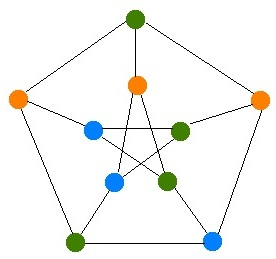
\includegraphics[scale=0.4]{seance8ex2}
     \end{center}
    \item  $\mathcal{X} = 2$ car ce graphe est biparti.
  \end{enumerate}
\end{solution}

\paragraph{3. } Vrai ou faux? \\
\begin{enumerate}[(a)]
  \item Un graphe de degré maximum 3 peut être colorié avec 4 couleurs.
  \item Un graphe de degré maximum 4 peut être colorié avec 4 couleurs.
  \item Si $G$ contient $K_n$ comme sous-graphe, alors son nombre chromatique est supérieur ou égal à $n$.
  \item Si $G$ est de nombre chromatique égal à $n$, alors $G$ contient $K_n$ comme sous-graphe.
\end{enumerate}

\begin{solution}
  \begin{enumerate}
    \item Vrai car $\mathcal{X} \leq$ degré max $+ 1 = 4$. 
    \item  Pas toujours. Le graphe $K_5$ en nécessite $5$ par exemple.
    \item Vrai puisqu'on aura déjà besoin de $5$ pour colorier $K_n$.
    \item Faux. Prenons par exemple un pentagone. Son nombre chromatique est égal à $3$ sans pour qu'il ne contienne de triangle. En fait, dès qu'on aura un cycle de longueur impaire, on va avoir $n \geq 3 $ sans pour autant que le graphe ne contienne $K_n$.
  \end{enumerate}
\end{solution}

\paragraph{4. } L'algorithme glouton de coloration associé à un graphe $G$ fonctionne comme suit: on parcourt les sommets $v_1,v_2,…,v_n$ de $G$ dans un ordre fixé arbitrairement. Lorsqu'on rencontre le sommet $v_i$, on lui assigne la plus petite couleur qui n'est pas encore utilisée par un de ses voisins.
\begin{enumerate}[(a)]
  \item Montrez que tout graphe $G$ possède une séquence de sommets pour laquelle l'algorithme glouton utilise un nombre minimum de couleurs.
  \item Construisez pour tout $k \geq 1$ un arbre de degré maximum $k$ et une séquence de ses sommets pour laquelle l'algorithme glouton utilise $k+1$ couleurs.
\end{enumerate}

\begin{solution}
  \begin{enumerate}
    \item En partant du graphe colorié, on peut créer une telle séquence en mettant d'abord tous les sommets de couleur $1$, puis tous les sommets de couleur $2$, etc. Le graphe obtenu à l'aide de l'algorithme glouton sera peut-être différent de celui qu'on avait au départ dans le sens où cet algorithme assigne la couleur la plus petite possible donc il se peut par exemple qu'il y a un noeud de couleur $2$ qui devienne de couleur $1$. L'algorithme glouton utilisera cependant bien le nombre minimal de couleurs, ce qui est bien ce qu'on veut!
    \item  Soit $A_1$ un noeud isolé. On peut ensuite créer $A_k$, avec $k \geq 2$, en créant un noeud relié à toutes les structures créées précédemment. La figure  ci-dessous illustre une telle construction.
    \begin{center}
    	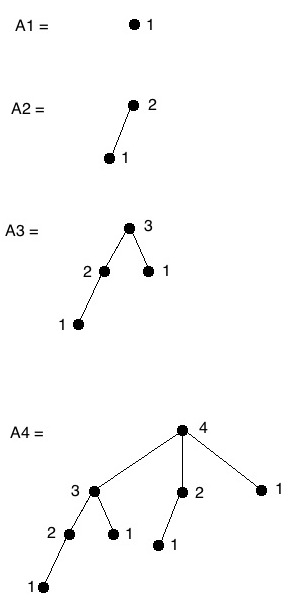
\includegraphics[scale=0.6]{seance8ex4}
     \end{center}
  \end{enumerate}
\end{solution}


\paragraph{5. } Pour les deux graphes ci-dessous appliquez l'algorithme de coloration glouton, et trouvez $\chi(G)$.


\begin{figure}[h!]
  \centering
  %\begin{center}
  \subfigure[]{
    \begin{tikzpicture}[-,>=stealth',shorten >=1pt,auto]
      \Vertex[x=0 ,y=0]{1}
      \Vertex[x=1 ,y=1]{2}
      \Vertex[x=2,y=0]{3}
      \Vertex[x=1 ,y=-1]{4}
      \Vertex[x=3 ,y=1]{5}
      \Vertex[x=3 ,y=-1]{6}
      \Vertex[x=4 ,y=0]{7}



      \path[every node/.style={font=\sffamily\small}]
      (1) edge node [left] {} (2)
      edge node [left] {} (5)
      edge node [left] {} (3)
      edge node [left] {} (4)
      edge node [left] {} (6)

      (2) edge node [right] {} (3)
      edge node [right] {} (7)
      edge node [right] {} (5)

      (3) edge node [right] {} (4)
      edge node [left] {} (5)
      edge node [left] {} (6)
      edge node [left] {} (7)

      (4) edge node [right] {} (6)
      edge node [right] {} (7)

      (5) edge node [right] {} (7)

      (6) edge node [right] {} (7);

  \end{tikzpicture} }
  \subfigure[]{
    \begin{tikzpicture}[-,>=stealth',shorten >=1pt,auto]
      \Vertex[x=0 ,y=0]{1}
      \Vertex[x=1 ,y=1]{2}
      \Vertex[x=1,y=0]{3}
      \Vertex[x=1 ,y=-1]{4}
      \Vertex[x=3 ,y=1]{5}
      \Vertex[x=3 ,y=-1]{6}
      \Vertex[x=2 ,y=0]{7}

      \path[every node/.style={font=\sffamily\small}]
      (1) edge node [left] {} (2)
      edge node [left] {} (3)
      edge node [left] {} (4)

      (2) edge node [right] {} (3)
      edge node [right] {} (7)
      edge node [right] {} (5)

      (3) edge node [right] {} (4)
      edge node [left] {} (7)

      (4) edge node [right] {} (6)
      edge node [right] {} (7)

      (5) edge node [right] {} (7)
      edge node [right] {} (6)

      (6) edge node [right] {} (7);

    \end{tikzpicture}
  }

\end{figure}

\begin{solution}
  \begin{enumerate}
    \item 
    \begin{itemize}
    \item noeud 1 $\Rightarrow$ couleur 1
    \item noeud 2 $\Rightarrow$ couleur 2
    \item noeud 3 $\Rightarrow$ couleur 3
    \item noeud 4 $\Rightarrow$ couleur 2
    \item noeud 5 $\Rightarrow$ couleur 4
    \item noeud 6 $\Rightarrow$ couleur 4
    \item noeud 7 $\Rightarrow$ couleur 1
    \end{itemize}
    Comme $K_4$ est inclus dans le graphe, on doit avoir $\mathcal{X} \geq 4$  et donc on a effectivement bien $\mathcal{X} = 4$.
    \item
    \begin{itemize}
    \item noeud 1 $\Rightarrow$ couleur 1
    \item noeud 2 $\Rightarrow$ couleur 2
    \item noeud 3 $\Rightarrow$ couleur 3
    \item noeud 4 $\Rightarrow$ couleur 2
    \item noeud 5 $\Rightarrow$ couleur 1
    \item noeud 6 $\Rightarrow$ couleur 3
    \item noeud 7 $\Rightarrow$ couleur 4
    \end{itemize}
    Regardons le cycle 23465. Puisqu'il est de longueur impaire, il va falloir 3 couleurs pour le colorier. Ensuite, on aura besoin d'une autre couleur pour le noeud $7$ comme il est relié à tous les noeuds du cycle. Dès lors, on a effectivement bien $\mathcal{X} = 4$ .
     \end{enumerate}
\end{solution}

\paragraph{6. } Sous quelle condition la somme des coefficients d'un polynôme chromatique est-elle nulle?
\begin{solution}
  La somme des coefficients du polynôme $= \pi_G(1)$ et $\pi_G(1) = 0$ veut dire que G a au moins une arête.
\end{solution}

\paragraph{7. } Trouvez le polynôme chromatique du graphe biparti complet $K_{2,2}$, et donnez le nombre de colorations possibles du cycle $C_4$ avec 5 couleurs.
\begin{solution}
  \begin{enumerate}
  \item En utilisant le fait que $\pi_k(G) = \pi_k(G-e) - \pi_k(G.e)$, on trouve que $\pi_k(K_{2,2}) = k^2(k-1)^2 - k (k-1)^2 - k(k-1)(k-2) = k^4-4k^3+6k^2-3k$.
  \item $C_4$ et $K_{2,2}$ sont isomorphes donc ils ont le même polynôme chromatique et $\pi_5(C_4) = \pi_5(K_{2,2}) = 5^4 - 4\cdot 5^3 + 6\cdot 5^2 - 3\cdot 5 = 260$.
\end{enumerate}
\end{solution}

\paragraph{8. }
\begin{enumerate}[(a)]
  \item Trouvez le polynôme chromatique d'un graphe chemin de longueur $n$
  \item Utilisez ce résultat pour trouver le polynôme chromatique d'un graphe circuit de longueur $n$.
\end{enumerate}
\begin{solution}
  \begin{enumerate}
  \item On démontre par récurrence que $p_k(P_n) = k(k-1)^n$.
  \item Etant donné que $\pi_k(G) = \pi_k(G-e) - \pi_k(G.e)$, on peut écrire que
           \begin{eqnarray*}
           p_k(C_n) &=& p_k(P_{n-1}) - p_k(C_{n-1})\\
           		    &=& k(k-1)^{n-1} - k(k-1)^{n-2} + ... + k(k-1)\\
		             &=& k(k-1) [(k-1)^{n-2} - (k-1)^{n-3} + ... + (-1)^n]\\
		             &=& k(k-1)\frac{1}{k}[(k-1)^{n-1}+(-1)^n]\\
		             &=& (k-1)^n + (-1)^n (k-1)
	   \end{eqnarray*}             
\end{enumerate}
\end{solution}

\paragraph{9. } Soit le graphe parallélépipède $3 \times 3 \times 2$.

\begin{enumerate}[(a)]
  \item Chaque arête du graphe est de longueur 1. On souhaite décrire un chemin qui part du sommet $s$ et arrive au sommet $t$ en passant au moins une fois par chaque arête. Quelle est la longueur minimale d'un tel chemin?
  \item Quel est le nombre minimum de couleurs nécessaires pour colorier les sommets de façon à ce que deux sommets adjacents soient toujours de couleurs différentes?
  \item Soit $P_G(k)$ le polynôme chromatique de ce graphe. Quel est le degré de $P_G(k)$? Que vaut $P_G(2)$?
  \item Trouvez une expression aussi explicite que possible pour le nombre de chemins de longueur $k$ du sommet $s$ à lui-même.
\end{enumerate}

\begin{figure}[h!]
  \centering
  %\includegraphics[scale=0.7]{img_tp8.jpg}
\end{figure}
